%\documentclass[11pt]{beamer}
\documentclass[11pt, handout]{beamer}

% Allgemeine Definitionen
\usepackage[english]{babel}	% Deutsche Sprachanpassung, z.B. Silbentrennung bei Worten mit Sonderzeichen
\usepackage[utf8]{inputenc}		% Direkte Eingabe von Umlauten

\usepackage{multimedia}		% Animations-Unterstützung (braucht hyperref | hyperref ist Teil von beamer )
\usepackage{xcolor}
\usepackage{fancyvrb}


% Verschiedene Operatoren
\newcommand{\union}{\ensuremath{\cup}}		% Die Vereinigung
\newcommand{\schnitt}{\ensuremath{\cap}}		% Der Schnitt
\newcommand{\und}{\ensuremath{\wedge}}		% Das und-Symbol
\newcommand{\oder}{\ensuremath{\vee}}		% Das oder-Symbol
\newcommand{\folgt}[1]{\ensuremath{\stackrel{#1}{\Rightarrow}}}	% Das Folgerungszeichen mit Symbol darüber 
\newcommand{\gleich}[1]{\ensuremath{\stackrel{#1}{=}}}	% Das Gleichheitszeichen mit Symbol darüber 
\newcommand{\isdef}{\ensuremath{\mathrel{\mathop:}=}}		% Das "ist-definiert"-Zeichen
\newcommand{\defis}{\ensuremath{=\mathrel{\mathop:}}}		% Das "ist-definiert"-Zeichen (andersrum)

% Weiterer nützlicher Kram
%\usepackage{enumitem}		% NICHT kompatibel mit beamer!
\usepackage{amsfonts, amsmath, amssymb}
\usepackage{amsthm}			% Eigene Umgebungen
\usepackage{thumbpdf}	% Seitenvorschau in PDF-Dokumenten

\usepackage{nicefrac}

\usepackage{pgf, tikz}
\usetikzlibrary{arrows, decorations.pathreplacing, calc, decorations.pathmorphing, shapes}

% Erst die Farbe (optional), dann die Norm, dann der Inhalt
\newcommand{\norm}[3][black]{\ensuremath{\left\Vert #3\right\Vert_{\textcolor{#1}{#2}}}}

% Die folgenden Befehle dienen dazu, verschiedene Konventionen darzustellen. Man kann damit
% auf einfache Weise die in dem Dokument verwendeten Konventionen umschalten.

%\newcommand{\bisn}[1]{\ensuremath{\underline{#1}}}	% Bezeichnung für die Menge {1,..,n}
\newcommand{\bisn}[1]{\ensuremath{\{1,\dots , #1 \}}}	% Alternative (ohne Fallunterscheidung)

% Das Erzeugnis, das erste Argument zeigt an, welches Erzeugnis gemeint ist, das zweite gibt seinen Inhalt an.
%\newcommand{\spn}[2][]{\ensuremath{\mathrm{span} \{ #1 \}}}
\newcommand{\spn}[2][]{\ensuremath{\left\langle #2 \right\rangle _{ #1 }}}

\newcommand{\grad}[1]{\ensuremath{\mathrm{grad}( #1 )}}
%\newcommand{\grad}[1]{\ensuremath{\nabla #1}}

\newcommand{\tr}[1]{\ensuremath{#1^{tr}}} % Bezeichnung für die Transponierte einer Matrix

% Die Mengentheoretische Differenz
\newcommand{\ohne}{\ensuremath{-}}
%\newcommand{\ohne}{\ensuremath{\backslash}}

\DeclareMathOperator{\Hom}{Hom}
\DeclareMathOperator{\GL}{GL}
\DeclareMathOperator{\diag}{diag}
\DeclareMathOperator{\Rg}{Rang}
\DeclareMathOperator{\Bild}{Bild}
\DeclareMathOperator{\Kern}{Kern}
\DeclareMathOperator{\Spur}{Spur}
\DeclareMathOperator{\Aut}{Aut}
\DeclareMathOperator{\Sym}{Sym}
\DeclareMathOperator{\Pot}{Pot}
\DeclareMathOperator{\Grad}{Grad}
\DeclareMathOperator{\kgV}{kgV}

\newcommand{\menge}[1]{\ensuremath{\mathbb{#1}}}
\newcommand{\N}{\menge{N}}
\newcommand{\Z}{\menge{Z}}
\newcommand{\Q}{\menge{Q}}
\newcommand{\R}{\menge{R}}
\newcommand{\C}{\menge{C}}

% Mit den schönen Buchstaben arbeiten
\renewcommand{\phi}{\varphi}

\renewcommand{\subset}{\subseteq}

% Verschiedene mögliche Umgebungen
\newtheorem{lem}{Lemma}[section]		% Lemma
\newtheorem{bsp}[lem]{Beispiel}		% Beispiel
\newtheorem{folg}[lem]{Folgerung}	% Folgerung
\newtheorem{bem}[lem]{Bemerkung}
\newtheorem{satz}[lem]{Satz}			% Satz
\newtheorem{kor}[lem]{Korollar}		% Korollar
%\newtheorem{alg}[lem]{Algorithmus}	% Algorithmus
%\theoremstyle{definition}
\newtheorem{defi}[lem]{Definition}	% Definition
\theoremstyle{remark}
\newtheorem*{idea}{Beweisidee}	% Beweisidee (vor dem eigentlichen Beweis)




\beamertemplatenavigationsymbolsempty

\usetheme{Madrid}
%	AnnArbor | Antibes | Bergen |
%	Berkeley | Berlin | Boadilla |
%	boxes | CambridgeUS | Copenhagen |
%	Darmstadt | default | Dresden |
%	Frankfurt | Goettingen |Hannover |
%	Ilmenau | JuanLesPins | Luebeck |
%	Madrid | Malmoe | Marburg |
%	Montpellier | PaloAlto | Pittsburgh |
%	Rochester | Singapore | Szeged |
%	Warsaw
%\usecolortheme{seahorse}
%	albatross | beaver | beetle |
%	crane | default | dolphin |
%	dove | fly | lily | orchid |
%	rose |seagull | seahorse |
%	sidebartab | structure |
%	whale | wolverine
%\usefonttheme{professionalfonts}
%	default | professionalfonts | serif |
%	structurebold | structureitalicserif |
%	structuresmallcapsserif
%\useinnertheme{rounded}
%	circles | default | inmargin |
%	rectangles | rounded
%\useoutertheme{shadow}
%	default | infolines | miniframes |
%	shadow | sidebar | smoothbars |
%	smoothtree | split | tree

% Graphic support
\newcommand{\primaryBlue}{blue}
\newcommand{\primaryRed}{red}
\newcommand{\primaryGreen}{green!60!black}


\newcommand{\colorVertex}{\primaryBlue}
\newcommand{\colorEdge}{black}
\newcommand{\colorFace}{yellow}
\newcommand{\colorEdgeBack}{\primaryBlue!20!white}

\newcommand{\colorVertexNode}{magenta!50!white}

\newcommand{\colorEdgeA}{\primaryBlue}
\newcommand{\colorEdgeB}{\primaryRed}
\newcommand{\colorEdgeC}{\primaryGreen}


\newcommand{\colorFaceA}{cyan}
\newcommand{\colorFaceB}{magenta}
\newcommand{\colorFaceC}{orange}

\newcommand{\colorRed}{\primaryRed}

\newcommand{\colorGraphA}{black}
\newcommand{\colorGraphB}{\primaryBlue}
\newcommand{\colorGraphC}{\primaryRed}

\newcommand{\colorGraphAlpha}{\primaryRed}
\newcommand{\colorGraphBeta}{black}
\newcommand{\colorGraphGamma}{\primaryBlue}
\newcommand{\colorGraphDelta}{\primaryGreen}

% This document contains the TikZ-header for all our LaTeX-computations.
% It especially contains all global graphic parameters.

\usepackage{amsmath, amssymb, amsfonts} % Standard Math-stuff

\usepackage{tikz}
\usetikzlibrary{calc}
\usetikzlibrary{positioning}

% Define a text=none option for nodes that ignores the given text, from
% https://tex.stackexchange.com/questions/59354/no-text-none-in-tikz
\makeatletter
\newif\iftikz@node@phantom
\tikzset{
  phantom/.is if=tikz@node@phantom,
  text/.code=%
    \edef\tikz@temp{#1}%
    \ifx\tikz@temp\tikz@nonetext
      \tikz@node@phantomtrue
    \else
      \tikz@node@phantomfalse
      \let\tikz@textcolor\tikz@temp
    \fi
}
\usepackage{etoolbox}
\patchcmd\tikz@fig@continue{\tikz@node@transformations}{%
  \iftikz@node@phantom
    \setbox\pgfnodeparttextbox\hbox{}
  \fi\tikz@node@transformations}{}{}
\makeatother

% Now we define the global styles
% The global styles are defined nestedly. You have to give your tikzpicture
% the global options [vertexStyle, edgeStyle, faceStyle] to activate them.
% 
% You can disable labels by using the option nolabels, i.e. 
% vertexStyle=nolabels to deactivate vertex labels.
%
% If you want to have a specific style for your picture, you can also use
% this specific meta-style instead of the general style. For example if you
% want to use double edges in one single picture - no matter the style of
% the rest of the document - you can use edgeDouble instead of edgeStyle.
%
% To set the default style, modify the vertexStyle/.default entry.

% Vertex styles
\tikzset{ 
    vertexNodePlain/.style = {fill=gray, shape=circle, inner sep=0pt, minimum size=2pt, text=none},
    vertexPlain/labels/.style = {
        vertexNode/.style={vertexNodePlain},
        vertexLabel/.style={gray}
    },
    vertexPlain/nolabels/.style = {
        vertexNode/.style={vertexNodePlain},
        vertexLabel/.style={text=none}
    },
    vertexPlain/.style = vertexPlain/#1,
    vertexPlain/.default=labels
}
\tikzset{
    vertexNodeNormal/.style = {fill=blue, shape=circle, inner sep=0pt, minimum size=4pt, text=none},
    vertexNormal/labels/.style = {
        vertexNode/.style={vertexNodeNormal},
        vertexLabel/.style={blue}
    },
    vertexNormal/nolabels/.style = {
        vertexNode/.style={vertexNodeNormal},
        vertexLabel/.style={text=none}
    },
    vertexNormal/.style = vertexNormal/#1,
    vertexNormal/.default=labels
}
\tikzset{
    vertexNodeBall/.style = {shape=circle, ball color=orange, inner sep=2pt, outer sep=0pt, minimum size=3pt},
    vertexBall/labels/.style = {
        vertexNode/.style={vertexNodeBall, text=black},
        vertexLabel/.style={text=none}
    },
    vertexBall/nolabels/.style = {
        vertexNode/.style={vertexNodeBall, text=none},
        vertexLabel/.style={text=none}
    },
    vertexBall/.style = vertexBall/#1,
    vertexBall/.default=labels
}
\tikzset{ 
    vertexStyle/.style={vertexNormal=#1},
    vertexStyle/.default = labels
}


% 1) position of the vertex
% 2) relative position of the node
% 3) name of the vertex
\newcommand{\vertexLabelR}[3]{
    \node[vertexLabel, #2] at (#1) {#3};
}
% 1) position of the vertex
% 2) absolute position of the node
% 3) name of the vertex
\newcommand{\vertexLabelA}[3]{
    \node[vertexLabel] at (#2) {#3};
}


% Edge styles
% If you have trouble with the double-lines overlapping, this might (?) help:
% https://tex.stackexchange.com/questions/288159/closing-the-ends-of-double-line-in-tikz
\tikzset{
    edgeLinePlain/.style={line join=round},
    edgePlain/labels/.style = {
        edge/.style={edgeLinePlain},
        edgeLabel/.style={fill=blue!20!white}
    },
    edgePlain/nolabels/.style = {
        edge/.style={edgeLinePlain},
        edgeLabel/.style={text=none}
    },
    edgePlain/.style = edgePlain/#1,
    edgePlain/.default = labels
}
\tikzset{
    edgeLineDouble/.style = {thin, double=gray!90!white, double distance=.3pt, line join=round},
    edgeDouble/labels/.style = {
        edge/.style = {edgeLineDouble},
        edgeLabel/.style = {fill=blue!20!white}
    },
    edgeDouble/nolabels/.style = {
        edge/.style = {edgeLineDouble},
        edgeLabel/.style = {text=none}
    },
    edgeDouble/.style = edgeDouble/#1,
    edgeDouble/.default = labels
}
\tikzset{
    edgeStyle/.style = {edgePlain=#1},
    edgeStyle/.default = labels
}

% Face styles
% Here we have an exception - the style face is always defined.
% 
\newcommand{\faceColorY}{yellow!60!white}   % yellow
\newcommand{\faceColorB}{blue!60!white}     % blue
\newcommand{\faceColorP}{cyan!60}           % purple
\newcommand{\faceColorR}{red!60!white}      % red
\newcommand{\faceColorG}{green!60!white}    % green
\newcommand{\faceColorO}{orange!50!yellow!70!white} % orange

\newcommand{\faceColor}{\faceColorY}
\newcommand{\faceColorSwap}{\faceColorB}
\tikzset{
    face/.style = {fill=#1},
    face/.default = \faceColor,
    faceY/.style = {face=\faceColorY},
    faceB/.style = {face=\faceColorB},
    faceP/.style = {face=\faceColorP},
    faceR/.style = {face=\faceColorR},
    faceG/.style = {face=\faceColorG},
    faceO/.style = {face=\faceColorO}
}
\tikzset{
    faceStyle/labels/.style = {
        faceNode/.style = {}
    },
    faceStyle/nolabels/.style = {
        faceNode/.style = {text=none}
    },
    faceStyle/.style = faceStyle/#1,
    faceStyle/.default = labels
}
\tikzset{ face/.style={fill=#1} }
\tikzset{ faceSwap/.code=
    \ifdefined\swapColours
        {face=\faceColorSwap}
    \else
        {face=\faceColor}
    \fi
}

% Sometimes we want to implement different behaviour for the generated 
% HTML-pictures (for example, shading is not supported in HTML).
% For that we define a macro to check whether we run the code with
% htlatex. The code comes from 
% https://tex.stackexchange.com/questions/93852/what-is-the-correct-way-to-check-for-latex-pdflatex-and-html-in-the-same-latex
\makeatletter
\edef\texforht{TT\noexpand\fi
  \@ifpackageloaded{tex4ht}
    {\noexpand\iftrue}
    {\noexpand\iffalse}}
\makeatother


\usepackage{hyperref}



\author[Baumeister]{Markus Baumeister\\ \vspace{1mm} \small{(j/w Alice Niemeyer)}}
\title{Simplicial surfaces in GAP}
\institute[Aachen]{Lehrstuhl B für Mathematik\\RWTH Aachen University}
\date{30.08.2017}

\begin{document}

% Titelseite
\begin{frame}
\titlepage
\end{frame}


\begin{frame}
    \tableofcontents[pausesections]
\end{frame}


%%%%%%%%%%%%%%%%%%%%%%%%%%%%%%%%%%%%%%%%%%%%%%%%%%%
%%
%%    First section
%%
\section{General simplicial surfaces}
\frame{\tableofcontents[currentsection]}

\begin{frame}
    \frametitle{Motivation}
    \pause
    Goal: simplicial surfaces (and generalisations) in GAP
    \pause
    \begin{center}
                            \begin{tikzpicture}[vertexPlain=nolabels, edgeStyle=nolabels, faceStyle=nolabels]
                        % We need to define the drawing style
	
		        % First a tetrahedron
		        \begin{scope}[xshift=0cm]
			    \coordinate (A) at (0,0);
			    \coordinate (B) at (2,0);
		    	    \coordinate (C) at (0.8,1.5);
			    \coordinate (D) at (1.9,0.7);
			
                            \draw[face,edge]
                                (A) -- (B) -- (C) -- cycle
                                (B) -- (C) -- (D) -- cycle;
			    \draw[dashed,edge] (A) -- (D);
		        \end{scope}
		
		        % Second: four triangles in the form of a cone
		        \begin{scope}[xshift=3cm]
                            			    \coordinate (A) at (0,0);
			    \coordinate (B) at (1.7,0.5);
			    \coordinate (C) at (1.3,1.4);
			    \coordinate (D) at (0.5,1.5);
			    \coordinate (E) at (1,0.7);
			
			    % Take care to draw the faces in the back first
                            \draw[face,edge]
                                (A) -- (B) -- (C) -- cycle
                                (A) -- (C) -- (D) -- cycle;
                            \draw[face,edge]
                                (A) -- (B) -- (E) -- cycle
                                (A) -- (E) -- (D) -- cycle;
                            \draw[edge, dashed] (A) -- (C);

		        \end{scope}
		
		        % Three triangles that share an edge
		        \begin{scope}[xshift=7cm]
                            \coordinate (A) at (0,0);
\coordinate (B) at (0,1.5);
\coordinate (C) at (-0.7,0.4);
\coordinate (D) at (0.8,0.4);
\coordinate (E) at (0.9,0.8);
			
\draw[edge, face]
    (A) -- (B) -- (E) -- cycle;
\draw[edge,face]
    (A) -- (B) -- (C) -- cycle
    (A) -- (B) -- (D) -- cycle;
\draw[edge, dashed] (A) -- (E);
		     

		        \end{scope}
		
		        % A butterfly of triangles
		        \begin{scope}[xshift=10cm]
                            \def\LUX{-0.8}
\def\LUY{-0.3}
\def\LMX{-1.2}
\def\LMY{0.5}
\def\LOX{-0.5}
\def\LOY{1}
\coordinate (A) at (0,0);
\coordinate (B) at (\LUX,\LUY);
\coordinate (C) at (\LMX,\LMY);
\coordinate (D) at (\LOX,\LOY);
\coordinate (E) at (-\LOX,\LOY);
\coordinate (F) at (-\LMX,\LMY);
\coordinate (G) at (-\LUX,\LUY);
			
\draw[face,edge]
    (A) -- (B) -- (C) -- cycle
    (A) -- (C) -- (D) -- cycle;
\draw[faceSwap, edge]
    (A) -- (E) -- (F) -- cycle
    (A) -- (F) -- (G) -- cycle;

\foreach \p/\r/\n in {A/below/1, D/above/2, C/left/3, B/below/4, G/below/5, F/right/6, E/above/7}{
    \vertexLabelR{\p}{\r}{\n}
}

\foreach \p/\q/\n in {B/C/III, C/D/I, F/G/IV, E/F/II}{
    \node[faceLabel] at (barycentric cs:A=1,\p=1,\q=1) {\n};
}

		        \end{scope}
		
		        % An open cone of two triangles
		        \begin{scope}[xshift=1cm, yshift=-3cm]
			    \coordinate (A) at (0,0);
			    \coordinate (B) at (1.3,0.4);
			    \coordinate (C) at (0.4,1.3);
			
                            \draw[face, edge]
                                (A) -- (B) to[bend right=45] (C) -- cycle
                                (A) -- (B) to[bend left=45] (C) -- cycle;
		        \end{scope}
		
		        % A surface from non-triangular shapes
		        \begin{scope}[xshift=4cm, yshift=-3cm]
			    \coordinate (A) at (0,0);
			    \coordinate (B) at (1,0);
			    \coordinate (C) at (0.5,0.6);
			    \coordinate (D) at (0,1);
			    \coordinate (E) at (0.5,1.3);
			    \coordinate (F) at (1,1);
			    \coordinate (G) at (1.7,0.8);
			    \coordinate (H) at (1.8,0.2);
			
                            \draw[face, edge]
                                (A) -- (B) -- (C) -- cycle
                                (A) -- (C) -- (D) -- cycle
                                (D) -- (C) -- (F) -- (E) -- cycle
                                (C) -- (F) -- (G) -- (H) -- (B) -- cycle;
		        \end{scope}

                        % Double tetrahedron
                        \begin{scope}[xshift=8.7cm, yshift=-2.3cm, scale=0.5]
                            % First tetrahedron is ABCD, second one is DEFG
\coordinate (A) at (-3,-1);
\coordinate (B) at (-1,-1.5);
\coordinate (C) at (-2,1);
\coordinate (D) at (0,0);
\coordinate (E) at (3,-0.1);
\coordinate (F) at (1.5,2);
\coordinate (G) at (1.2,1);

\filldraw[face] (A) -- (B) -- (C) -- cycle;
\filldraw[face] (B) -- (C) -- (D) -- cycle;
\filldraw[faceAlt] (D) -- (F) -- (E) -- cycle;

\draw[dashed] (A) -- (D);
\draw[dashed] (E) -- (G);
\draw[dashed] (D) -- (G);
\draw[dashed] (F) -- (G);

                        \end{scope}
                    \end{tikzpicture}
 

    \end{center}
    \pause
    $\leadsto$ examples of \textbf{polygonal complexes}
\end{frame}

\begin{frame}
    \frametitle{No embedding}
    \pause
    We do \textbf{not} work with embeddings (mostly) in $\R^3$
    \begin{itemize}
        \pause
        \item are very hard to compute \pause (compare the pentagon flippy)
        \pause
        \item are often unknown for an abstractly constructed surface
        \pause
        \item are mostly independent from \textit{intrinsic structure}
        \pause
        \item[$\Rightarrow$] lengths and angles are not important
        \pause
        \item[$\leadsto$] incidence structure is intrinsic
    \end{itemize}
\end{frame}

\begin{frame}[fragile]
    % The option is needed: https://tex.stackexchange.com/questions/119309/arguments-of-tikzset-inside-a-beamer-document
    \frametitle{Incidence structure of a polygonal complex}
    \onslide<2->{
        A \textbf{polygonal complex} consists of
    }
    
    \begin{itemize}
        \item<3-> set of vertices $\mathcal{V}$ \hfill
            \onslide<4->{
                \begin{tikzpicture}
                    \newcommand{\vertexDot}[2]{
                        % xshift, label
                        \coordinate[label={[\vertexColor]right:#2}] (V#2) at (#1,0);
                        \fill[vertex] (V#2) circle (\vSize);
                    }

                    \onslide<4-9>{
                        \vertexDot{0}{2}
                    }
                    \onslide<4-13>{
                        \vertexDot{1}{3}
                        \vertexDot{2}{5}
                    }
                    \onslide<4-14>{
                        \vertexDot{3}{7}
                    }
                    \onslide<4-19>{
                        \vertexDot{4}{11}
                    }
                \end{tikzpicture}
            }
        \item<5-> set of edges $\mathcal{E}$ \hfill
            \onslide<6->{
                {\small
                \begin{tikzpicture}[scale=0.9]
                    \newcommand{\storedEdge}[2]{
                        \coordinate (A#2) at (-0.6+#1*1.5, -0.3);
                        \coordinate (B#2) at (0.6+#1*1.5, 0.3);
                        \draw[edge] (A#2) -- (B#2);
                        \drawEdge{A#2}{B#2}{#2}
                    }

                    \onslide<6-9>{
                        \storedEdge{0}{6}
                    }
                    \onslide<6-12>{
                        \storedEdge{1}{8}
                        \storedEdge{2}{9}
                    }
                    \onslide<6-16>{
                        \storedEdge{3}{10}
                    }
                    \onslide<6-19>{
                        \storedEdge{4}{12}
                        \storedEdge{5}{13}
                    }
                \end{tikzpicture}
                }
            }
        \item<7-> set of faces $\mathcal{F}$ \hfill
            \onslide<8->{
                {\small
                
\begin{tikzpicture}[scale=0.9,
                        decoration={snake, amplitude=0.5, segment length=4.5}]
                    \onslide<8-10>{
                        \node at (0,0) {1};
                        \draw[decorate] (0,0) circle (0.3);
                    }
                    \onslide<8-18>{
                        \node at (2,0) {4};
                        \draw[decorate] (2,0) circle (0.3);
                    }
                \end{tikzpicture}
                }
            }
        \item<9-> transitive relation \def\brSize{\big}
            $\subset \brSize(\mathcal{V} \times \mathcal{E} \brSize)
            \uplus \brSize(\mathcal{V} \times \mathcal{F} \brSize)
            \uplus \brSize(\mathcal{E} \times \mathcal{F} \brSize)$
    \end{itemize}
    % Draw the pictures
    \onslide<10->{
        \begin{tikzpicture}[vertexNode/.style={circle, draw=\vertexColor}, node distance=0.5]

            % Edge nodes
            \node[edgeBackground] (E6) {6};
            \uncover<13->{
                \node[edgeBackground] (E8) [right=of E6] {8};
                \node[edgeBackground] (E9) [right=of E8] {9};
            }
            \uncover<17->{
                \node[edgeBackground] (E10) [right=of E9] {10};
            }
            \uncover<20->{
                \node[edgeBackground] (E12) [right=of E10] {12};
                \node[edgeBackground] (E13) [right=of E12] {13};
            }

            % Face nodes
            \uncover<11->{
                \node (F1) [above=of E8] {1};
                \draw (F1) -- (E6);
            }
            \uncover<13->{
                \draw (E8) -- (F1);
                \draw (E9) -- (F1);
            }

            \node (Help) at ($(E10)!0.5!(E12)$) {};
            \uncover<19->{
                \node (F4) [above=of Help] {4};
                \draw (F4) -- (E9);
                \draw (F4) -- (E10);
            }
            \uncover<20->{
                \draw (E12) -- (F4) -- (E13); 
            }

            % Vertex nodes
            \uncover<15->{
                \node[vertexNode] (V7) [below=of Help] {7};
            }
            \uncover<17->{
                \draw (E10) -- (V7);
            }
            \uncover<20->{
                \draw (E13) -- (V7);
            }

            \uncover<20->{
                \node[vertexNode] (V11) [right=of V7] {11}
                    edge (E13) edge (E12);
            }

            \uncover<14->{
                \node[vertexNode] (V5) [left=of V7] {5}
                    edge (E8) edge (E9);
                \node[vertexNode] (V3) [left=of V5] {3}
                    edge (E6) edge (E9);
            }
            \uncover<20->{
                \draw (E12) -- (V5);
            }
            \uncover<17->{
                \draw (E10) -- (V3);
            }

            \uncover<10->{
                \node[vertexNode] (V2) [left=of V3] {2}
                    edge (E6);
            }
            \uncover<13->{
                \draw (E8) -- (V2);
            }

            \begin{scope}[xshift=7cm, yshift=-0.6cm, scale=0.7]
                %       P3 ------------ P4
                %      / |       10     | 
                %    6/  |              |
                %    /   |              |
                %  P1  1 |9      4      |13
                %    \   |              |
                %    8\  |              |
                %      \ |        12    |
                %       P2 ------------ P5

                \uncover<10->{
                    \coordinate[label={[vertex]left:2}] (P1) at (0,0.5);
                }
                \uncover<14->{
                    \coordinate[label={[vertex]below:5}] (P2) at (2,-1);
                    \coordinate[label={[vertex]above:3}] (P3) at (2,2);
                }
                \uncover<15->{
                    \coordinate[label={[vertex]above:7}] (P4) at (5,2);
                }
                \uncover<20->{
                    \coordinate[label={[vertex]below:11}] (P5) at (5,-1);
                }

                % Draw first face
                \onslide<11-12>{
                    \fill[\faceColor] (P1) -- (P2) -- (P3) -- cycle;
                    \node at ($1/3*(P1)+1/3*(P2)+1/3*(P3)$) {1};
                }
                \onslide<13->{
                    \filldraw[face] (P1) -- (P2) -- (P3) -- cycle;
                    \node at ($1/3*(P1)+1/3*(P2)+1/3*(P3)$) {1};
                }
                \onslide<10-12>{
                    \draw[\edgeColor] (P1) -- (P3);
                }

                % Draw the second face
                \onslide<19>{
                    \fill[\faceColor] (P2) -- (P3) -- (P4) -- (P5) -- cycle;
                    \node at ($1/4*(P2)+1/4*(P3)+1/4*(P4)+1/4*(P5)$) {4};
                }
                \onslide<17-19>{
                    \draw[\edgeColor] (P2) -- (P3) -- (P4);
                }
                \onslide<20->{           
                    \filldraw[face] (P2) -- (P3) -- (P4) -- (P5) -- cycle;
                    \node at ($1/4*(P2)+1/4*(P3)+1/4*(P4)+1/4*(P5)$) {4};
                }
        

                % Draw the edges
                \onslide<10->{
                    \drawEdge{P1}{P3}{6}
                }
                \onslide<13->{
                    \drawEdge{P1}{P2}{8}
                    \drawEdge{P2}{P3}{9}
                }
                \onslide<17->{
                    \drawEdge{P3}{P4}{10}
                }
                \onslide<20->{
                    \drawEdge{P4}{P5}{13}
                    \drawEdge{P5}{P2}{12}
                }

                % Draw the concrete points
                \onslide<10->{
                    \fill[vertex] (P1) circle (\vSize);
                }
                \onslide<14->{
                    \fill[vertex] (P2) circle (\vSize);
                    \fill[vertex] (P3) circle (\vSize);
                }
                \onslide<15->{
                    \fill[vertex] (P4) circle (\vSize);
                }
                \onslide<20->{
                    \fill[vertex] (P5) circle (\vSize);
                }
            \end{scope}
        \end{tikzpicture}
    }
    \begin{enumerate}
        \item<12-> Every face is a polygon
        \item<16-> Every vertex lies in an edge \onslide<18->{and every edge lies in a face}
    \end{enumerate}
\end{frame}


\begin{frame}{Isomorphism testing}
    \pause
    Incidence geometry allows ``easy" isomorphism testing.
    \pause
    Incidence structure can be interpreted as a coloured graph:
    \pause
        \begin{center}
        \begin{tikzpicture}[vertexNode/.style={circle,
            fill=\colorVertexNode}, node distance=0.5]
            % Edge nodes
            \node[edgeBackground] (E6) {6};
            \node[edgeBackground] (E8) [right=of E6] {8};
            \node[edgeBackground] (E9) [right=of E8] {9};
            \node[edgeBackground] (E10) [right=of E9] {10};
            \node[edgeBackground] (E12) [right=of E10] {12};
            \node[edgeBackground] (E13) [right=of E12] {13};

            % Face nodes
            \node[fill=\colorFace] (F1) [above=of E8] {1}
                edge (E6) edge (E8) edge (E9);
            \node (Help) at ($(E10)!0.5!(E12)$) {};
            \node[fill=\colorFace] (F4) [above=of Help] {4}
                edge (E9) edge (E10) edge (E12) edge (E13);

            % Vertex nodes
            \node[vertexNode] (V7) [below=of Help] {7}
                edge (E10) edge (E13);
            \node[vertexNode] (V11) [right=of V7] {11}
                edge (E13) edge (E12);
            \node[vertexNode] (V5) [left=of V7] {5}
                edge (E8) edge (E9) edge (E12);
            \node[vertexNode] (V3) [left=of V5] {3}
                edge (E6) edge (E9) edge (E10);
            \node[vertexNode] (V2) [left=of V3] {2}
                edge (E6) edge (E8);
        \end{tikzpicture}
        \end{center}
    \pause
    $\leadsto$ reduce to graph isomorphism problem

    \pause
    $\leadsto$ can be solved quite easily by \texttt{Nauty} (McKay, Piperno)

    \pause
    Interfaced by NautyTracesInterface (by Gutsche, Niemeyer, Schweitzer)
    \begin{itemize}
        \pause
        \item direct C--interface without writing files
        \pause
        \item also returns automorphism group
    \end{itemize}
\end{frame}


\begin{frame}{General properties}
    \pause
    Some properties can be computed for all polygonal complexes:
    \pause
    \begin{itemize}
        \item Connectivity
        \pause
        \item Euler--Characteristic
    \end{itemize}
    \pause
    \textit{Orientability} is \textbf{not} one of them.
    \pause
    Counterexample:
        \begin{center}
            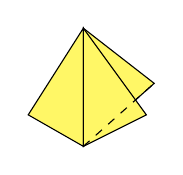
\begin{tikzpicture}
                \coordinate (A) at (0,0);
                \coordinate (B) at (0,1.5);
                \coordinate (C) at (-0.7,0.4);
                \coordinate (D) at (0.8,0.4);
                \coordinate (E) at (0.9,0.8);
                			
                % draw back face first
                \filldraw[face] (A) -- (B) -- (E) -- cycle;
                % Now draw front faces
                \filldraw[face] (A) -- (B) -- (C) -- cycle;
                \filldraw[face] (A) -- (B) -- (D) -- cycle;
                % Draw dashed line
                \draw[dashed] (A) -- (E);
	    \end{tikzpicture}
        \end{center}
    \pause
    $\Rightarrow$ every edge lies in at most two faces (for well--definedness)
    
    \pause
    $\leadsto$ \textbf{ramified polygonal surfaces}
\end{frame}


\begin{frame}{Why ramified?}
    \pause
    Typical example of ramified polygonal surface:
    \pause
    \begin{center}
        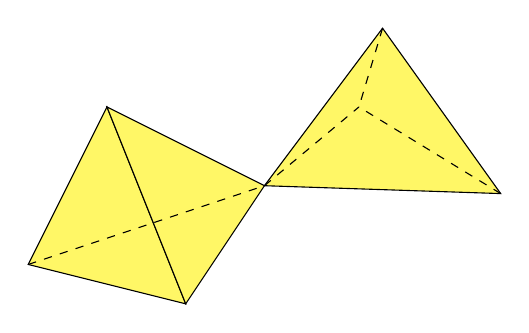
\begin{tikzpicture}
                % First tetrahedron is ABCD, second one is DEFG
                \coordinate (A) at (-3,-1);
                \coordinate (B) at (-1,-1.5);
                \coordinate (C) at (-2,1);
                \coordinate (D) at (0,0);
                \coordinate (E) at (3,-0.1);
                \coordinate (F) at (1.5,2);
                \coordinate (G) at (1.2,1);
                
                \filldraw[face] (A) -- (B) -- (C) -- cycle;
                \filldraw[face] (B) -- (C) -- (D) -- cycle;
                \filldraw[face] (D) -- (F) -- (E) -- cycle;
                
                \draw[dashed] (A) -- (D);
                \draw[dashed] (E) -- (G);
                \draw[dashed] (D) -- (G);
                \draw[dashed] (F) -- (G);
        \end{tikzpicture}
    \end{center}
    \pause
    $\Rightarrow$ It is not a surface -- there is a \textit{ramification} at 
        the central vertex
    
    \pause
    A \textbf{polygonal surface} does not have these ramifications.
\end{frame}



            
%%%%%%%%%%%%%%%%%%%%%%%%%%%%%%%%%%%%%%%%%%%%%%%%%%%%%%%%%%
%%
%%              Second section
%%
\section{Edge colouring and group properties}
\newcommand{\colA}{\colorEdgeA}
\newcommand{\colB}{\colorEdgeB}
\newcommand{\colC}{\colorEdgeC}
\newcommand{\width}{very thick}
\frame{\tableofcontents[currentsection]}


\begin{frame}{Embedding questions}
    \uncover<2->{
        Given: A polygonal complex
    }
    \begin{itemize}
        \item<3-> Can it be embedded?
        \item<4-> In how many ways?
    \end{itemize}
    \uncover<5->{
        Simplifications:
    }
    \begin{enumerate}
        \item<6-> Only polygonal surfaces (that are built from polygons)
        \item<7-> All polygons are triangles (\textbf{simplicial surfaces})
        \item<8-> All triangles are isometric
    \end{enumerate}
    \uncover<10->{
        $\leadsto$ Edge--colouring encodes different lengths
    }
    \uncover<9->{
            \begin{center}
                %       F
                %    C     E 
                % A     B    D
                \begin{tikzpicture}[scale=0.9]
                    \coordinate (A) at (0,0);
                    \coordinate (B) at (3,0);
                    \coordinate (C) at (1,1);
                    \coordinate (D) at ($2*(B)$);
                    \coordinate (E) at ($(B)+(C)$);
                    \coordinate (F) at ($2*(C)$);

                    \only<9>{
                        \draw (A) -- (B) -- (D) -- (E) -- (B) -- (C) -- (E) -- (F) -- (C) -- (A);
                    }

                    \uncover<10->{
                        \draw[\colA, \width] (A) -- (B) -- (D);
                        \draw[\colA, \width] (C) -- (E);
                        \draw[\colB, \width] (B) -- (C);
                        \draw[\colB, \width] (D) -- (E) -- (F);
                        \draw[\colC, \width] (A) -- (C) -- (F);
                        \draw[\colC, \width] (B) -- (E);
                    }
                \end{tikzpicture}
            \end{center}
    }
\end{frame}


\begin{frame}{Colouring as permutation}
    \onslide<2->{
        Consider tetrahedron \onslide<4->{with edge colouring}
    }
    \begin{center}
        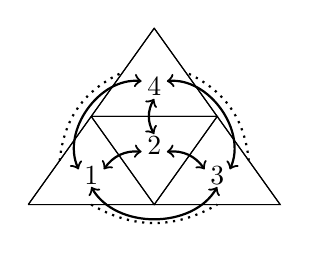
\begin{tikzpicture}[scale=0.8]
                \coordinate (A) at (0,0);
                \coordinate (B) at (2,0);
                \coordinate (C) at (1,1.4);
                \coordinate (D) at ($2*(B)$);
                \coordinate (E) at ($(B)+(C)$);
                \coordinate (F) at ($2*(C)$);
            \onslide<3->{
                \draw (A) -- (B) -- (D) -- (E) -- (F) -- (C) -- (E) -- (B) -- (C) -- (A);
                \node at (barycentric cs:A=1,B=1,C=1) {1};
                \node at (barycentric cs:B=1,C=1,E=1) {2};
                \node at (barycentric cs:B=1,D=1,E=1) {3};
                \node at (barycentric cs:C=1,E=1,F=1) {4};
                \draw[dotted,thick] ($(A)!0.5!(C)$) to[bend left] ($(C)!0.5!(F)$);
                \draw[dotted,thick] ($(A)!0.5!(B)$) to[bend right] ($(B)!0.5!(D)$);
                \draw[dotted,thick] ($(D)!0.5!(E)$) to[bend right] ($(E)!0.5!(F)$);
            }
            \onslide<5->{
                \draw[\colA, \width] (A) -- (B) -- (D);
                \draw[\colA, \width] (C) -- (E);
                \draw[\colB, \width] (B) -- (C);
                \draw[\colB, \width] (D) -- (E) -- (F);
                \draw[\colC, \width] (A) -- (C) -- (F);
                \draw[\colC, \width] (B) -- (E);
            }

            % Draw switching arrows
            \onslide<9-11>{
                \draw[<->,\colB, thick] (barycentric cs:A=1,B=2,C=2) to[bend left] (barycentric cs:B=2,C=2,E=1);
            }
            \onslide<10-11>{
                \draw[<->,\colB,thick] (barycentric cs:B=1,D=2,E=2) to[bend right=60] (barycentric cs:E=2,F=2,C=1);
            }
            \onslide<12>{
                \draw[<->,\colA,thick] (barycentric cs:A=2,B=2,C=1) to[bend right=60] (barycentric cs:B=2,D=2,E=1);
                \draw[<->,\colA,thick] (barycentric cs:C=2,E=2,B=1) to[bend left] (barycentric cs:C=2,E=2,F=1);
            }
            \onslide<13>{
                \draw[<->,\colC,thick] (barycentric cs:A=2,B=1,C=2) to[bend left=60] (barycentric cs:C=2,E=1,F=2);
                \draw[<->,\colC,thick] (barycentric cs:B=2,C=1,E=2) to[bend left] (barycentric cs:B=2,D=1,E=2);
            }
        \end{tikzpicture}
    \end{center}
    \onslide<6->{
        \textit{simplicial surface} $\Rightarrow$ \onslide<7->{at most two faces at each edge}
    
        \begin{itemize}
            \item<8->[$\leadsto$] every edge defines transposition of incident faces
            \item<11->[$\leadsto$] every colour class defines permutation of the faces
            \item<9-> \textcolor{\colB}{(1,2)}\onslide<10->{\textcolor{\colB}{(3,4)}}
                    \onslide<12->{, \textcolor{\colA}{(1,3)(2,4)}}
                    \onslide<13->{, \textcolor{\colC}{(1,4)(2,3)}}
            \item<14->[$\leadsto$] group theoretic considerations
                \begin{itemize}
                    \item<15-> The connected components of the surface correspond to 
                        \onslide<16->{the orbits of $\langle 
                            \textcolor{\colA}{\sigma_a}, 
                            \textcolor{\colB}{\sigma_b}, 
                            \textcolor{\colC}{\sigma_c}\rangle$ on
                        the faces}
                        \onslide<17->{
                            (fast computation for permutation groups)
                        }
                \end{itemize}
        \end{itemize}
    }
\end{frame}
         

\begin{frame}{How do faces fit together?}
    \onslide<2->{
        Consider a face of the surface \onslide<4->{and a neighbouring face}
    }

    \onslide<6->{
        The neighbour can be coloured in two ways:
    }
    \onslide<1->{
        \begin{center}
        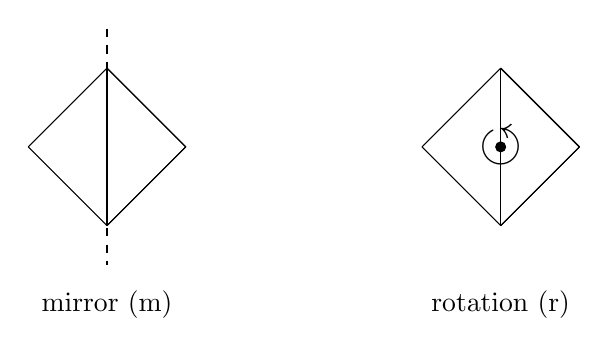
\begin{tikzpicture}
            % Numbers to determine drawing
            \def\x{1}
            \def\y{1}

            %      B
            %    / | \
            %   A  |  D
            %    \ | /
            %      C
            
            % First pair
            \begin{scope}
                \coordinate (A) at (0,0);
                \coordinate (B) at (\x,\y);
                \coordinate (C) at (\x,-\y);
                \coordinate (D) at (2*\x,0);

                \onslide<3->{
                    \draw[\colA,\width] (A) -- (B);
                    \draw[\colB,\width] (A) -- (C);
                    \draw[\colC,\width] (B) -- (C);
                }
                \onslide<5->{
                    \draw (B) -- (D) -- (C);
                }
                \onslide<7->{
                    \draw[\colA,\width] (B) -- (D);
                    \draw[\colB,\width] (C) -- (D);
                }
                \onslide<9->{
                    % Draw mirror line
                    \draw[dashed, thick] (\x,1.5*\y) -- (\x,-1.5*\y);
                    \node at (\x,-2*\y) {mirror (m)};
                }
            \end{scope}

            % Second pair
            \begin{scope}[xshift=5cm]
                \coordinate (A) at (0,0);
                \coordinate (B) at (\x,\y);
                \coordinate (C) at (\x,-\y);
                \coordinate (D) at (2*\x,0);

                \onslide<6->{
                    \draw[\colA,\width] (A) -- (B);
                    \draw[\colB,\width] (A) -- (C);
                    \draw[\colC,\width] (B) -- (C);
                    \draw (B) -- (D) -- (C);
                }
                \onslide<8->{
                    \draw[\colB,\width] (B) -- (D);
                    \draw[\colA,\width] (C) -- (D);
                }
                \onslide<10->{
                    % Draw rotation center and circle
                    \fill[black] (\x,0) circle (2pt);
                    \node[scale=2] at (\x,0) {$\circlearrowleft$};
                    \node at (\x,-2*\y) {rotation (r)};
                }
            \end{scope}
        \end{tikzpicture}
        \end{center}
    }
    \onslide<11->{
        This gives an \textbf{mr--assignment} for the edges.
    }

    \onslide<12->{
        Permutations and mr--assignment uniquely determine the surface.
    }
\end{frame}


\begin{frame}{Constructing surfaces from groups}
    \pause
    A general mr--assignment leads to complicated surfaces.
    
    \pause
    Simplification: edges of same colour have the same type

    \pause
    Example
        \begin{center}
            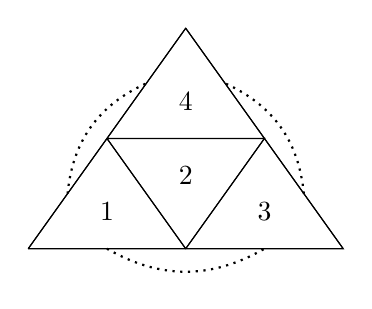
\begin{tikzpicture}
                \coordinate (A) at (0,0);
                \coordinate (B) at (2,0);
                \coordinate (C) at (1,1.4);
                \coordinate (D) at ($2*(B)$);
                \coordinate (E) at ($(B)+(C)$);
                \coordinate (F) at ($2*(C)$);

                \draw (A) -- (B) -- (D) -- (E) -- (F) -- (C) -- (E) -- (B) -- (C) -- (A);
                \node at (barycentric cs:A=1,B=1,C=1) {1};
                \node at (barycentric cs:B=1,C=1,E=1) {2};
                \node at (barycentric cs:B=1,D=1,E=1) {3};
                \node at (barycentric cs:C=1,E=1,F=1) {4};
                
                \draw[dotted,thick] ($(A)!0.5!(C)$) to[bend left] ($(C)!0.5!(F)$);
                \draw[dotted,thick] ($(A)!0.5!(B)$) to[bend right] ($(B)!0.5!(D)$);
                \draw[dotted,thick] ($(D)!0.5!(E)$) to[bend right] ($(E)!0.5!(F)$);

                \draw[\colA, \width] (A) -- (B) -- (D);
                \draw[\colA, \width] (C) -- (E);
                \draw[\colB, \width] (B) -- (C);
                \draw[\colB, \width] (D) -- (E) -- (F);
                \draw[\colC, \width] (A) -- (C) -- (F);
                \draw[\colC, \width] (B) -- (E);
            \end{tikzpicture}
        \end{center}
    \pause
    has only r--edges.
\end{frame}


\begin{frame}{The mirror--case}
    \pause
    If all edges are mirrors, the situation is simple.
    \pause
    \begin{lem}
        A simplicial surface has only mirror--edges iff it covers a 
        single triangle\pause, i.\,e. there is a surjective incidence--preserving
        map \pause to the simplicial surface consisting of exactly one face.
    \end{lem}
    \pause
    Consider
        \begin{center}
            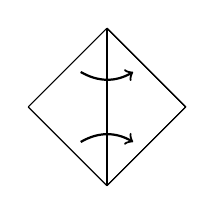
\begin{tikzpicture}
                \def\x{1}
                \def\y{1}

                \coordinate (A) at (0,0);
                \coordinate (B) at (\x,\y);
                \coordinate (C) at (\x,-\y);
                \coordinate (D) at (2*\x,0);

                    \draw[\colA,\width] (A) -- (B);
                    \draw[\colB,\width] (A) -- (C);
                    \draw[\colC,\width] (B) -- (C);
                    \draw (B) -- (D) -- (C);
                    \draw[\colA,\width] (B) -- (D);
                    \draw[\colB,\width] (C) -- (D);

                \def\mid{3}
                \def\near{5}
                \draw[->,thick] (barycentric cs:A=\mid,B=\near,C=1) to[bend right] (barycentric cs:B=\near,C=1,D=\mid);
                \draw[->,thick] (barycentric cs:A=\mid,B=1,C=\near) to[bend left] (barycentric cs:B=1,C=\near,D=\mid);
            \end{tikzpicture}
        \end{center}
    \begin{itemize}
        \pause
        \item[$\Rightarrow$] Unique map that preserves incidence
        \pause
        \item Covering pulls back a mirror--colouring of the triangle.
        \pause
        \item Mirror--colouring defines a map to the triangle.
    \end{itemize}
\end{frame}


\begin{frame}[fragile]{Construction from permutations}
    \onslide<2->{
        Start with three involutions 
        \textcolor{\colA}{$\sigma_a$}, 
        \textcolor{\colB}{$\sigma_b$}, \textcolor{\colC}{$\sigma_c$} 
        in permutation representation
        \onslide<3->{(like generators of a finite group)}
    }

    \onslide<4->{
    \begin{lem}
        There exists a coloured surface with the given involutions
        \onslide<5->{where all edges are mirror edges.}
    \end{lem}
    }

    \begin{itemize}
        \item<6-> The faces are the points moved by the involutions
        \item<7-> The edges are the cycles of the involutions
        \item<8-> The vertices are \onslide<11->{the orbits of 
            $\langle \textcolor{\colA}{\sigma_a}, 
            \textcolor{\colB}{\sigma_b} \rangle$
            on the faces} \onslide<12->{(for all pairs)}
    \end{itemize}

    \onslide<9->{
    \begin{center}
    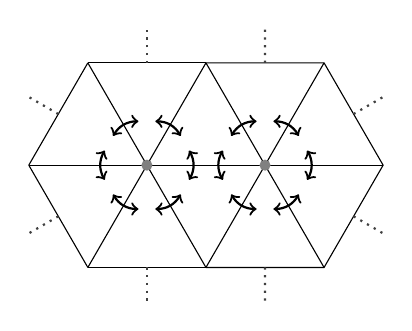
\begin{tikzpicture}
        %     P2 ---- P1 ---- Q3
        %    /  \    /  \   /  \
        %   /    \  /    \ /    \
        % P3 ---- Z ---- P0 ---- Q2
        %   \    /  \    /  \   /
        %    \  /    \  /    \ /
        %     P4 ---- P5 ---- Q1

        % Define the coordinates
        \def\rad{1.5}
        \coordinate (Z) at (0,0);
        \foreach \i in {0,1,2,3,4,5}
            \coordinate (P\i) at (60*\i:\rad);

        \foreach \i in {1,2,3}
            \coordinate (Q\i) at ($(P0) + (-120+60*\i:\rad)$);
        
        % Draw the circle around Z
        \foreach \i/\j in {0/1, 1/2, 2/3, 3/4, 4/5, 5/0}{
            \draw[\colC, \width] (P\i) -- (P\j);
        }

        % Draw the spokes of Z
        \foreach \i in {0,2,4}
            \draw[\colA,\width] (Z) -- (P\i);

        \foreach \i in {1,3,5}
            \draw[\colB,\width] (Z) -- (P\i);

        % Draw missing lines around P0
        \draw[\colB, \width] (P5) -- (Q1) -- (Q2) -- (Q3) -- (P1);
        \draw[\colA, \width] (Q1) -- (P0) -- (Q3);
        \draw[\colC, \width] (P0) -- (Q2);

        % Draw the continuations
        \foreach \p/\q/\z in {P1/P2/Z, P2/P3/Z, P3/P4/Z, P4/P5/Z, P5/Q1/P0, Q1/Q2/P0, Q2/Q3/P0, Q3/P1/P0}
            \draw[gray!50!black, dotted, thick] ($(\p)!0.5!(\q)$) -- (barycentric cs:\z=-0.5,\p=1,\q=1);

        % Draw the vertices
        \foreach \p in {Z,P0}
            \fill[gray] (\p) circle (2pt);

        % Draw the arc segments (center, outer, first, second, colour)
        \newcommand{\arcSeg}[5]{
            \draw[#5, thick, <->] (barycentric cs:#1=4,#2=2,#3=1) to[bend right] (barycentric cs:#1=4,#2=2,#4=1);
        }
        \onslide<10->{
        \arcSeg{Z}{P1}{P0}{P2}{\colB}
        \arcSeg{Z}{P2}{P1}{P3}{\colA}
        \arcSeg{Z}{P3}{P2}{P4}{\colB}
        \arcSeg{Z}{P4}{P3}{P5}{\colA}
        \arcSeg{Z}{P5}{P4}{P0}{\colB}
        \arcSeg{Z}{P0}{P5}{P1}{\colA}
        }

        \onslide<12->{
        \arcSeg{P0}{Q3}{Q2}{P1}{\colA}
        \arcSeg{P0}{P1}{Q3}{Z}{\colC}
        \arcSeg{P0}{Z}{P1}{P5}{\colA}
        \arcSeg{P0}{P5}{Z}{Q1}{\colC}
        \arcSeg{P0}{Q1}{P5}{Q2}{\colA}
        \arcSeg{P0}{Q2}{Q1}{Q3}{\colC}
        }
    \end{tikzpicture}
    \end{center}
    }
\end{frame}


\begin{frame}[fragile]{Construction example}
    \onslide<2->{ $\textcolor{\colA}{\sigma_a} = \textcolor{\colA}{(1,2)(3,4)(5,6)(7,8)}$\\ }
    \onslide<3->{ $\textcolor{\colB}{\sigma_b} = \textcolor{\colB}{(1,4)(2,3)(5,8)(6,7)}$\\ }
    \onslide<4->{ $\textcolor{\colC}{\sigma_c} = \textcolor{\colC}{(1,5)(2,6)(3,7)(4,8)}$\\ }

    \begin{center}
    \begin{tikzpicture}
        % Coordinates
        \coordinate (Z) at (0,0);
        \foreach \i in {0,1,2,3,4}
            \coordinate (P\i) at (60*\i:2);
        \foreach \i/\j in {0/1, 1/2, 2/3, 3/4}
            \coordinate (Q\i\j) at ($(P\i)+(P\j)$);

        \newcommand{\vertex}[1]{
            \fill[black] (#1) circle (3pt);
        }
        \newcommand<>{\vertArc}[3]{
            \def\dist{0.2}
            \onslide#4{
                \filldraw[draw=black, fill=black!50!white] (#1) -- 
                    ($(#1)!\dist!(#2)$) to[bend right=25] ($(#1)!\dist!(#3)$) -- cycle;
            }
        }

        % Draw the arcs first (since faces have to be drawn on top)
        
        % 1
        \vertArc<6-10>{Z}{P1}{P2}
        \vertArc<11-13>{P2}{Z}{P1}
        \vertArc<16>{P1}{P2}{Z}
        
        % 2
        \vertArc<7-10>{Z}{P2}{P3}
        \vertArc<11-13>{P2}{P3}{Z}
        \vertArc<14-15>{P3}{Z}{P2}

        % 3
        \vertArc<8-10>{Z}{P3}{P4}
        \vertArc<14-15>{P3}{P4}{Z}
        \vertArc<18>{P4}{Z}{P3}

        % 4
        \vertArc<9-10>{Z}{P0}{P1}
        \vertArc<16>{P1}{Z}{P0}
        \vertArc<18>{P0}{P1}{Z}

        % 5
        \vertArc<12-13>{P2}{P1}{Q12}
        \vertArc<16>{P1}{Q12}{P2}
        \vertArc<19>{Q12}{P2}{P1}

        % 6
        \vertArc<13>{P2}{Q23}{P3}
        \vertArc<14-15>{P3}{P2}{Q23}
        \vertArc<19>{Q23}{P3}{P2}

        % 7
        \vertArc<15>{P3}{Q34}{P4}
        \vertArc<18>{P4}{P3}{Q34}
        \vertArc<19>{Q34}{P4}{P3}

        % 8
        \vertArc<16>{P1}{P0}{Q01}
        \vertArc<18>{P0}{Q01}{P1}
        \vertArc<19>{Q01}{P1}{P0}


        % First vertex

        % 1
        \onslide<5->{
            \node at (barycentric cs:Z=1,P1=1,P2=1) {1};
            \draw[\colA,\width] (Z) -- (P2);
            \draw[\colB,\width] (Z) -- (P1);
            \draw[\colC,\width] (P1) -- (P2);
        }

        % 2
        \onslide<7->{
            \node at (barycentric cs:Z=1,P2=1,P3=1) {2};
            \draw[\colB,\width] (Z) -- (P3);
            \draw[\colC,\width] (P2) -- (P3);
        }

        % 3
        \onslide<8->{
            \node at (barycentric cs:Z=1,P3=1,P4=1) {3};
            \draw[\colC,\width] (P3) -- (P4);
            \draw[\colA,\width] (Z) -- (P4);
        }

        % 4
        \onslide<9->{
            \node at (barycentric cs:Z=1,P0=1,P1=1) {4};
            \draw[\colA,\width] (Z) -- (P0);
            \draw[\colC,\width] (P0) -- (P1);
        }

        \onslide<10->{
            \draw[\colA,\width,dotted] ($(Z)!0.5!(P4)$) to[bend right] ($(Z)!0.5!(P0)$);
        }

        \onslide<6-10>{
            \vertex{Z}
        }


        % Second vertex

        % 5
        \onslide<12->{
            \node at (barycentric cs:P1=1,P2=1,Q12=1) {5};
            \draw[\colB,\width] (P1) -- (Q12);
            \draw[\colA,\width] (P2) -- (Q12);
        }

        % 6
        \onslide<13->{
            \node at (barycentric cs:P2=1,P3=1,Q23=1) {6};
            \draw[\colA,\width] (P2) -- (Q23);
            \draw[\colA,\width,dotted] ($(P2)!0.5!(Q23)$) to[bend left] ($(P2)!0.5!(Q12)$);
            \draw[\colB,\width] (P3) -- (Q23);
        }

        \onslide<11-13>{
            \vertex{P2}
        }


        % Third vertex

        % 7
        \onslide<15->{
            \node at (barycentric cs:P3=1,P4=1,Q34=1) {7};
            \draw[\colB,\width] (P3) -- (Q34);
            \draw[\colB,\width,dotted] ($(P3)!0.5!(Q23)$) to[bend right] ($(P3)!0.5!(Q34)$);
            \draw[\colA,\width] (P4) -- (Q34);
        }

        \onslide<14-15>{
            \vertex{P3}
        }

        % Fourth vertex

        % 8
        \onslide<16->{
            \node at (barycentric cs:P0=1,P1=1,Q01=1) {8};
            \draw[\colB,\width] (P1) -- (Q01);
            \draw[\colB,\width,dotted] ($(P1)!0.5!(Q01)$) to[bend right] ($(P1)!0.5!(Q12)$);
            \draw[\colA,\width] (P0) -- (Q01);
        }
        \onslide<16>{
            \vertex{P1}
        }


        \onslide<17->{
            \draw[\colA,\width,dotted] ($(P0)!0.5!(Q01)$) to[bend left=60] ($(P4)!0.5!(Q34)$);
        }

        % Fifth vertex
        \onslide<18>{
            \vertex{P0}
            \vertex{P4}
        }

        % Sixth vertex
        \onslide<19>{
            \vertex{Q01}
            \vertex{Q12}
            \vertex{Q23}
            \vertex{Q34}
        }


        \begin{scope}[xshift=6cm]
            % Coordinates of octahedron
                \def\len{2} % The length of the base
                \def\h{1}   % \h*\len is the hight of the apex above the 
                            % center of the square
                \coordinate (Mid) at (0,0);
                \coordinate (Right) at (0.5*\len,0.3*\len);
                \coordinate (Left) at (-0.75*\len,0.25*\len);
                \coordinate (Back) at ($(Right)+(Left)$);
                \coordinate (Center) at ($(Left)!0.5!(Right)$);
                \coordinate (Up) at ($(Center)+(0,\h*\len)$);
                \coordinate (Down) at ($(Center)+(0,-\h*\len)$);

                \onslide<20->{
                    \draw[\colA,\width] (Up) -- (Mid) -- (Down);
                    \draw[\colA,\width,dashed] (Up) -- (Back) -- (Down);
                    \draw[\colB,\width] (Up) -- (Right) -- (Down) -- (Left) -- cycle;
                    \draw[\colC,\width] (Left) -- (Mid) -- (Right);
                    \draw[\colC,\width,dashed] (Left) -- (Back) -- (Right);

                    %\node at (barycentric cs:Mid=1,Down=1,Right=1) {1};
                    %\node at (barycentric cs:Mid=1,Down=1,Left=1) {2};
                    %\node at (barycentric cs:Mid=1,Up=1,Right=1) {5};
                    %\node at (barycentric cs:Mid=1,Up=1,Left=1) {6};
                    
                    % Vertices to hide drawing problems in edge meetings
                    \foreach \p in {Mid,Right,Left,Back,Up,Down}
                        \fill[gray] (\p) circle (1pt);
                }
        \end{scope}
    \end{tikzpicture}
    \end{center}
\end{frame}



%%%%%%%%%%%%%%%%%%%%%%%%%%%%%%%%%%%%%%%%%%%%%%%%%%%%%%%%%%%%%%
%%
%%    Third section
%%
\section{Abstract folding}
\frame{\tableofcontents[currentsection]}

\begin{frame}{What kind of folding?}
    \pause
    There are many different kinds of folding (e.\,g. Origami)

    \pause
    Here:
    \begin{itemize}
        \pause
        \item Folding of surface in $\R^3$
        \pause
        \item Fold only at given edges (no introduction of new folding edges)
        \pause
        \item Folding should be rigid (no curvature)
    \end{itemize}

    \pause
    Goal: Classify possible folding patterns (given a net)

    \pause
    \begin{center}
        \only<1-7>{
            \phantom{ 
                \movie[ height = 0.4\textwidth, width = 0.4\textwidth, autostart, loop ]{}{TorusNetz.mp4}
            }
        }
        \only<8>{
            \movie[ height = 0.4\textwidth, width = 0.4\textwidth, autostart, loop ]{}{TorusNetz.mp4}
        }
    \end{center}

\end{frame}


\begin{frame}{Why are embeddings hard?}
    \pause
    Ideally, we would like to have embeddings.
    
    \pause
    But we want to define folding independently from an embedding, since:

    \begin{itemize}
        \pause
        \item They are very hard to compute (even for small examples)
        \pause
        \item We can only show foldability for specific small examples
            \begin{itemize}
                \pause
                \item Usually using regularity (like crystallographic symmetry)
                \pause
                \item No general method
            \end{itemize}
        \pause
        \item It is very hard to define iterated folding in an embedding
    \end{itemize}

    \pause
    \begin{center}
        \only<1-8>{
            \phantom{
                \movie[ height = 0.4\textwidth, width = 0.4\textwidth, autostart, loop ]{}{TorusNetz.mp4}
            }
        }
        \only<9>{
            \movie[ height = 0.4\textwidth, width = 0.4\textwidth, autostart, loop ]{}{TorusNetz.mp4}
        }
    \end{center}

\end{frame}


\begin{frame}{Folding without embedding}
    \pause
    Central idea:
    \begin{itemize}
        \pause
        \item Don't model folding process (needs embedding)
        \pause
        \item Describe starting and final folding state
            \begin{itemize}
                \pause
                \item Only consider changes in the topology
                    \pause (like identification of faces)
                \pause
                \item allows abstraction from embedding
            \end{itemize}
    \end{itemize}

    % Use pentagon-flippy to illustrate incidence rigidity

    \pause
    $\leadsto$ Incidence geometry (polygonal complex/surface)

    \begin{itemize}
        \pause
        \item Captures some folding restrictions \pause (rigidity of tetrahedron)
        \pause
        \item Still needs a lot of refinement
    \end{itemize}
\end{frame}

\newcommand{\colFaceA}{\colorFaceA}
\newcommand{\colFaceB}{\colorFaceB}
\newcommand{\colFaceC}{\colorFaceC}

\begin{frame}{Important properties of folding}
    \begin{itemize}
        \item<2-> The class of surfaces is not closed under folding
        \item<3-> Folding can be undone by \textit{unfolding}
        \item<4-> Identification of two faces might force identification of two other faces
            \begin{itemize}
                \item<7-> Can apply to arbitrary many faces 
                \item<10-> The forced identification is not unique
                \item<14-|handout:2>[$\Rightarrow$] Identify only two faces at a time
                    \begin{itemize}
                        \item<16-|handout:2>[$\leadsto$] Relax the rigidity--constraint:
                        \item<17-|handout:2> Allow non--rigid configurations as transitional states
                    \end{itemize}
            \end{itemize}
    \end{itemize}

    \begin{overlayarea}{\textwidth}{0.3\textwidth}
        \begin{center}
            \only<5-7,14|handout:0>{
                % First identification
                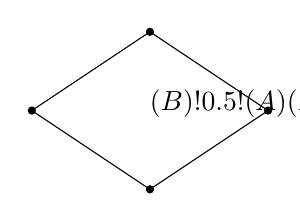
\begin{tikzpicture}
                    \def\Hdist{1.5}
	    	    \def\Vdist{1}
			
		    \coordinate (A) at (-\Hdist,0);
		    \coordinate (B) at (0,\Vdist);
		    \coordinate (C) at (\Hdist,0);
		    \coordinate (D) at (0,-\Vdist);
                    \draw (A) -- (B) -- (C) -- (D) -- cycle;

		    \foreach \p in {A,B,C,D}
		        \fill [\vertexColor] (\p) circle (1.5pt);
                    \planEdge{\colorRed,thick}{($(B)!0.5!(A)$)}{(barycentric cs:A=2,B=1,C=1,D=1)}{($(D)!0.5!(A)$)}
                    \uncover<6-7>{
                        \planEdge{\colorRed,thick}{($(B)!0.5!(C)$)}{(barycentric cs:A=1,B=1,C=2,D=1)}{($(D)!0.5!(C)$)}
                    }
                \end{tikzpicture}
            }

            % Arbitrary many faces
            \only<8-10|handout:0>{
                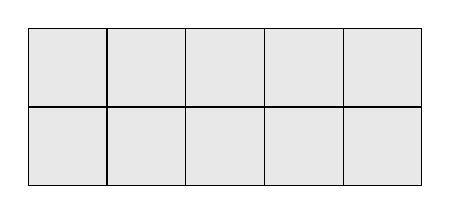
\begin{tikzpicture}
		    \foreach \i/\j in {1/0, 2/1, 3/2, 4/3, 5/4}
		    {
		        \filldraw [fill=black!9!white] (\j,0) -- (\i,0) -- (\i,1) -- (\j,1) -- cycle;
		        \filldraw [fill=black!9!white] (\j,0) -- (\i,0) -- (\i,-1) -- (\j,-1) -- cycle;
		    }
                    \uncover<9-10>{
                        \planEdge{\colorRed,thick}{(0.5,0.5)}{(0.75,0)}{(0.5,-0.5)}
	            }
                \end{tikzpicture}
            }

            % Picture of non-uniqueness:
            \only<11-13|handout:1>{
                \begin{tikzpicture}
                    \def\len{2}
                    \def\fak{0.7}
                    \coordinate (A) at (0,0);
                    \coordinate (B) at (\len,0);
                    \coordinate (C) at (\len,\len);
                    \coordinate (D) at (0,\len);
                    \coordinate (Back) at (0.2*\len,0.2*\len);

                    \behindPlane{Back}{A}{D}
                    \behindPlane{Back}{A}{B}

                    \behindPlane<11>[\colFaceB]{Back}{A}{60:\fak*\len}
                    \behindPlane<11>[\colFaceA]{Back}{B}{$(B)+(120:\fak*\len)$}

                    \behindPlane<12|handout:0>[\colFaceB]{Back}{A}{5:\fak*\len}
                    \behindPlane<12|handout:0>[\colFaceA]{Back}{B}{$(B)+(160:\fak*\len)$}

                    \behindPlane<13|handout:0>[\colFaceA]{Back}{B}{$(B)+(175:\fak*\len)$}
                    \behindPlane<13|handout:0>[\colFaceB]{Back}{A}{20:\fak*\len}

                    \planEdge[(Back)]{thick}{($(A)!0.5!(D)$)}{($(B)!0.7!(D)$)}{($(D)!0.5!(C)$)}

                    \behindPlane{Back}{C}{D}
                    \behindPlane{Back}{B}{C}

                \end{tikzpicture}
            }
            % 11: general picture
            % 12: First possible fold
            % 13: Second possible fold

            % Anomaly-picture
            \only<15-|handout:2>{
                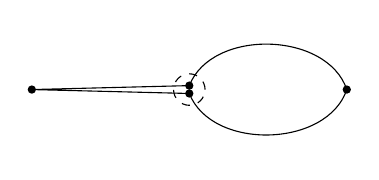
\begin{tikzpicture}
		    \def\r{2}	
		    \def\eps{0.05}
				
		    \coordinate (A) at (-\r,0);
		    \coordinate (B) at (0,\eps);
		    \coordinate (C) at (\r,0);
		    \coordinate (D) at (0,-\eps);
			
		    \draw (D) -- (A) -- (B);
		    \draw (B) to [bend left=70] (C);
		    \draw (D) to [bend right=70] (C);
			
		    \foreach \point in {A,B,C,D}
		        \fill [\vertexColor] (\point) circle (1.5pt);
				
		    \draw [dashed] (0,0) circle (0.2);
                \end{tikzpicture}
            }
        \end{center}
    \end{overlayarea}
\end{frame}


\begin{frame}{How to define abstract folding?}
    \uncover<2->{We need to define two structures:}
    \begin{enumerate}
        \item<3-> A folding state
            \begin{itemize}
                \item<5-> Based on polygonal complexes
                \item<6-> Describe ``is folded together" by an equivalence relation
                \item<7-> Describe order of faces in folding state
            \end{itemize}
        \item<4-> The folding steps
            \begin{itemize}
                \item<8-> Only two faces at a time
                \item<9-> Explain ``unordered folding" (e.\,g. covering)
                \item<10-> Modify to include face order relations
            \end{itemize}
    \end{enumerate}
\end{frame}


\begin{frame}{Unordered Folding (Covering)}
    \begin{center}
        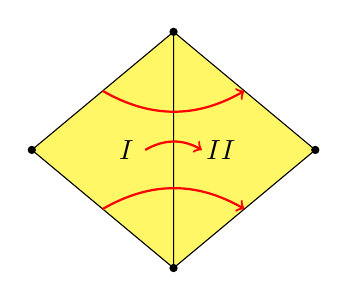
\begin{tikzpicture}
            \def\xOff{1.8}
            \def\yOff{1.5}

            %     B
            %   / | \
            % A   |   C
            %   \ | /
            %     D
            \coordinate (A) at (-\xOff,0);
            \coordinate (B) at (0,\yOff);
            \coordinate (C) at (\xOff,0);
            \coordinate (D) at (0,-\yOff);

            \uncover<3->{
                \filldraw[face] (A) -- (B) -- (D) -- cycle;
                \node at (barycentric cs:A=1,B=1,D=1) {$I$};
                \filldraw[face] (B) -- (C) -- (D) -- cycle;
                \node at (barycentric cs:B=1,C=1,D=1) {$II$};

                \foreach \p in {A,B,C,D}
                    \fill[\vertexColor] (\p) circle (1.5pt);
            }

            \uncover<5-7|handout:1>{
                \draw[\colorRed,thick,->] (barycentric cs:A=1,B=2,D=2) to[bend left] (barycentric cs:B=2,C=1,D=2);
                \draw[\colorRed,thick,->] ($(A)!0.5!(B)$) to[bend right] ($(B)!0.5!(C)$);
                \draw[\colorRed,thick,->] ($(A)!0.5!(D)$) to[bend left] ($(D)!0.5!(C)$);
            }
        \end{tikzpicture}
    \end{center}

    \begin{overprint}
        \onslide<1-7|handout:1>
        
        \uncover<2-7>{
            Why do we need more than a polygonal complex?
        }

        \uncover<4-7>{
            Naive folding definition: surjective map that respects incidence
        }

        \uncover<6-7>{
            Problem: Can't be unfolded
        }

        \uncover<7>{
            $\Rightarrow$ Folding state should not forget original structure
        }


        \onslide<8-16|handout:2>

        \uncover<8-16>{
            Represent folding by equivalence relation
            \begin{itemize}
                \item<9-> Separate relation on vertices, edges and faces
                \item<10-> Two elements are equivalent if they are folded together
                \item<11-> If two edges are equivalent, 
                    \uncover<12->{then their vertices have to be as well}
                    \uncover<13->{(likewise for faces)}
                \item<14-> The vertices of an edge are not equivalent
                    \uncover<15->{(likewise for faces)}
                \item<16->[$\Rightarrow$] Unordered folding is coarsening of equivalence relation
            \end{itemize}
        }
    \end{overprint}
\end{frame}


\begin{frame}{How does folding work?}
    \begin{enumerate}
        \item<2-> Choose two faces that are not folded together
        \item<4-> Choose how to identify them \uncover<6->{(like $I \sim II$ and $1 \sim 4$)}
        \item<7-> Add those pairs to the equivalence relation
    \end{enumerate}

    \begin{center}
        \begin{tikzpicture}
            \def\xOff{1.8}
            \def\yOff{1.5}

            %     B
            %   / | \
            % A   |   C
            %   \ | /
            %     D
            \uncover<3->{
                \coordinate[label={[vertex]left:1}] (A) at (-\xOff,0);
                \coordinate[label={[vertex]above:2}] (B) at (0,\yOff);
                \coordinate[label={[vertex]right:4}] (C) at (\xOff,0);
                \coordinate[label={[vertex]below:3}] (D) at (0,-\yOff);

                \filldraw[face] (A) -- (B) -- (D) -- cycle;
                \node at (barycentric cs:A=1,B=1,D=1) {$I$};
                \filldraw[face] (B) -- (C) -- (D) -- cycle;
                \node at (barycentric cs:B=1,C=1,D=1) {$II$};

                \foreach \p in {A,B,C,D}
                    \fill[\vertexColor] (\p) circle (1.5pt);
            }

            \uncover<5->{
                \draw[\colorRed,thick,->] (barycentric cs:A=1,B=2,D=2) to[bend left] (barycentric cs:B=2,C=1,D=2);
                \draw[\colorRed,thick,->] ($(A)!0.5!(B)$) to[bend right] ($(B)!0.5!(C)$);
                \draw[\colorRed,thick,->] ($(A)!0.5!(D)$) to[bend left] ($(D)!0.5!(C)$);
            }
        \end{tikzpicture}
    \end{center}

    \uncover<8->{Only restriction:}

    \uncover<9->{Two vertices in an edge can't be identified}
    \uncover<10->{(slightly generalized)}
\end{frame}


\begin{frame}[fragile]{Limitation of unordered folding}
    \pause
    We can't work with ordering of faces:
    \pause
    \begin{center}
        
\begin{tikzpicture}

            \newcommand{\plane}[3]{
                \def\len{1.5}
                \def\back{0.75}
                \def\xOff{0.5}
                \def\nOff{-0.3}
                
                \coordinate (Down) at (#1*\xOff,0);
                \coordinate (Up) at (#1*\xOff,\len);
                \coordinate (Back) at (\back*\xOff,\back*\xOff);

                \fill[#2] (Down) -- ($(Down)+(Back)$) -- ($(Up)+(Back)$) -- (Up) -- cycle;
                \node[#2] at (#1*\xOff,\nOff) {#3};
            }

            \plane{0}{\colFaceB}{1}
            \plane{1}{\colFaceA}{2}
            \plane{2}{\colFaceC}{3}

            % Second lines
            \begin{scope}[xshift=4cm]
                \plane{0}{\colFaceB}{1}
                \plane{1}{\colFaceC}{3}
                \plane{2}{\colFaceA}{2}
            \end{scope}
        \end{tikzpicture}
    \end{center}

    \pause
    Adding a linear order on each face equivalence class
    \pause is not enough:
    \pause
    \begin{center}
        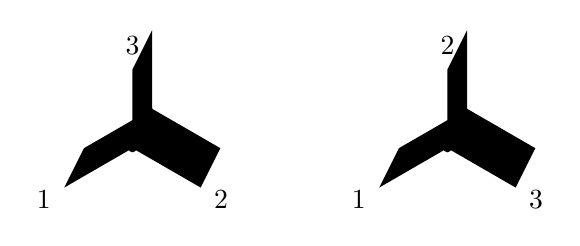
\begin{tikzpicture}

            \newcommand{\plane}[3]{
                \def\len{1}
                \def\nScale{1.3}

                \coordinate (Back) at (0.25*\len,0.5*\len);
                \fill[#2] (0,0) -- (#1:\len) -- +(Back) -- (Back) -- cycle; 
                \node[#2] at (#1:\nScale*\len) {#3};
                \draw (0,0) -- (Back);
            }

            \plane{210}{\colFaceA}{1}
            \plane{-30}{\colFaceB}{2}
            \plane{90}{\colFaceC}{3}

            \fill (0,0) circle (1.5pt);

            \begin{scope}[xshift=4cm]
                \plane{210}{\colFaceA}{1}
                \plane{-30}{\colFaceC}{3}
                \plane{90}{\colFaceB}{2}

                \fill (0,0) circle (1.5pt);
            \end{scope}
        \end{tikzpicture}
    \end{center}

    \pause
    $\leadsto$ define order of faces around edges
    \pause
    (we will skip the details)
\end{frame}


\begin{frame}{Folding complex}
    \pause
    \begin{defi}
        A \textbf{folding complex}
        \pause
        is a polygonal complex together with
        \begin{enumerate}
            \pause
            \item An equivalence relation on vertices, edges and faces
                \pause (``is folded together")
            \pause
            \item A linear ordering on each face equivalence class
            \pause
            \item A cyclical ordering of the faces around each edge equivalence class
        \end{enumerate}
        \pause
        such that the orderings are compatible
        \pause
        (in an appropriate sense).
    \end{defi}

    \pause
    To identify faces with each other, we have to combine those orderings.
    \begin{itemize}
        \pause
        \item linear orderings get concatenated
        \pause
        \item cyclical orderings are opened at one point
            \pause
            and combined
        \pause
        \item[!!] compatibility is not easily transfered,
            \pause
            but can be calculated
    \end{itemize}

\end{frame}


\begin{frame}[fragile]{Changed definition of folding}
    \begin{overprint}
        \only<2-4|handout:0>{Before (no ordering):}
        \only<5->{Folding with ordering:}
    \end{overprint}

    \begin{enumerate}
        \item<3-> Choose two faces that are not folded together
        \item<4-> Choose how to identify them and extend the equivalence relation
        \item<9-> Choose the sides of the faces that will meet
            \uncover<10->{and modify the orderings}
    \end{enumerate}

    \uncover<6->{
        $\leadsto$ Each face has two sides
    }

    \begin{center}
        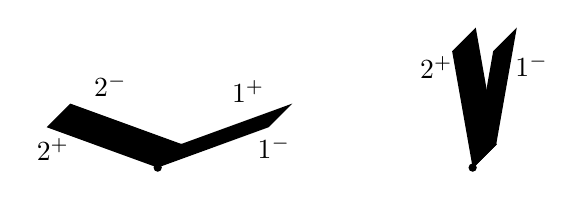
\begin{tikzpicture}
            \def\len{1.5}
            \def\wA{20}
            \def\wB{160}
            \def\nOff{10}

            % angle, colour
            \newcommand{\plane}[2]{
                \coordinate (Out) at (#1:\len);
                \coordinate (Back) at (0.2*\len,0.2*\len);

                \fill[#2] (0,0) -- (Out) -- +(Back) -- (Back) -- cycle;
                \draw (0,0) -- (Back);
            }

            \uncover<7->{
                \plane{\wA}{\colFaceA}
                \node[\colFaceA] at (\wA+2*\nOff:\len) {$1^+$};
                \node[\colFaceA] at (\wA-\nOff:\len) {$1^-$};

                \plane{\wB}{\colFaceB}
                \node[\colFaceB] at (\wB+\nOff:0.9*\len) {$2^+$};
                \node[\colFaceB] at (\wB-4*\nOff:0.8*\len) {$2^-$};

                \fill (0,0) circle (1.5pt);
            }

            \uncover<8->{
                \planEdge{}{(\wB-\nOff: 0.5*\len)}{(90:0.4*\len)}{(\wA+\nOff:0.5*\len)}
            }

            \begin{scope}[xshift=4cm]
                \uncover<8->{
                    \def\wA{80}
                    \def\wB{100}

                    \plane{\wB}{\colFaceB}
                    \node[\colFaceB] at (\wB+\nOff:0.9*\len) {$2^+$};
                    
                    \plane{\wA}{\colFaceA}
                    \node[\colFaceA] at (\wA-2*\nOff:\len) {$1^-$};

                    \fill (0,0) circle (1.5pt);
                }
            \end{scope}

        \end{tikzpicture}
    \end{center}

    \uncover<11->{
        $\Rightarrow$ Define folding by two face sides (\textbf{folding plan})
    }

    \uncover<12->{
        $\leadsto$ Allows reversible (un)folding
    }
\end{frame}


\begin{frame}[fragile]{Structure of multiple foldings}
    \uncover<2->{
        With folding plans we can perform the same folding in different folding complexes
    }
    \begin{center}
        
\begin{tikzpicture}
            \def\len{1.5}
            \def\off{10}

            %  B
            %   \
            %    Z -- C -- D
            %   /
            %  A
            \begin{scope}
                \coordinate (Z) at (0,0);
                \coordinate (A) at (-120:\len);
                \coordinate (B) at (120:\len);
                \coordinate (C) at (\len,0);
                \coordinate (D) at (2*\len,0);
                \coordinate (Back) at (-0.5*\len,0.25*\len);


                \uncover<3->{
                    \behindPlane{Back}{Z}{C}
                    \behindPlane{Back}{Z}{A}
                    \behindPlane{Back}{Z}{B}
                    \behindPlane{Back}{C}{D}
                    \foreach \p in {Z,A,B,C,D}
                        \fill[\vertexColor] (\p) circle (\vSize);
                }
                \uncover<5->{
                    \planEdge[(Back)]{\colorRed,thick}{(120+\off:0.5*\len)}{(180:0.5*\len)}{(-120-\off:0.5*\len)}
                }
            \end{scope}

            \begin{scope}[xshift=6cm]
                \def\pOff{0.1}

                \coordinate (Z) at (0,0);
                \coordinate (A) at (-120:\len);
                \coordinate (B) at (120:\len);
                \coordinate (C) at (\len,0);
                \coordinate (CAlt) at ($(C)+(0,0.5*\pOff)$);
                \coordinate (D) at (0.2*\len,\pOff);
                \coordinate (Back) at (-0.5*\len,0.25*\len);

                \uncover<4->{
                    \behindPlane{Back}{Z}{C}
                    \behindPlane{Back}{C}{$(C)+(0,\pOff)$}
                    \behindPlane{Back}{$(C)+(0,\pOff)$}{D}
                    \behindPlane{Back}{Z}{A}
                    \behindPlane{Back}{Z}{B}
                    \foreach \p in {A,B,Z,CAlt,D}
                        \fill[\vertexColor] (\p) circle (\vSize);
                }
                \uncover<6->{
                    \planEdge[(Back)]{\colorRed,thick}{(120+\off:0.5*\len)}{(180:0.5*\len)}{(-120-\off:0.5*\len)}
                }
            \end{scope}
        \end{tikzpicture}
    \end{center}

    \uncover<7->{
        $\leadsto$ more structure on the set of possible foldings
    }
\end{frame}


\begin{frame}[fragile]{Folding graph}
    \begin{itemize}
        \item<2->Vertices are folding complexes (modelling folding states)
        \item<3->Edges are folding plans connecting two folding complexes
    \end{itemize}

    \tikzset{graphVertex/.style={circle,fill=gray!70!white,inner sep=1.5pt}} %TODO make a better circle
    \begin{center}
        \begin{tikzpicture}[graphEdge/.style={thick}]
            \def\len{1.2}
            \def\off{10}
            \def\dist{0.5}

            \coordinate (Z) at (0,0);
            \coordinate (Back) at (0.4*\len,0.2*\len);
            \foreach \i in {0,1,2}
                \coordinate (P\i) at (120*\i:\len);


            \def\fgA{\colorGraphB}
            \def\fgB{\colorGraphA}
            \def\fgC{\colorGraphC}

            \planEdge<5->[(Back)]{graphEdge,\fgB}{(120+\off:0.5*\len)}{(180:\dist*\len)}{(240-\off:0.5*\len)}
            \behindPlane<4->{Back}{Z}{P2}
            \behindPlane<4->{Back}{Z}{P1}
            \planEdge<5->[(Back)]{graphEdge,\fgC}{(-120+\off:0.5*\len)}{(-60:\dist*\len)}{(-\off:0.5*\len)}
            \behindPlane<4->{Back}{Z}{P0}
            \planEdge<5->[(Back)]{graphEdge,\fgA}{(\off:0.5*\len)}{(60:\dist*\len)}{(120-\off:0.5*\len)}

            \uncover<4->{
                \foreach \i in {2,1,0}{
                    \fill[\vertexColor] (P\i) circle (1.5pt);
                }
            }

            \begin{scope}[xshift=3cm]
                \coordinate (Z) at (0,0);
                \coordinate (Back) at (0.4*\len,0.2*\len);
                \coordinate (P0) at (60-0.5*\off:\len);
                \coordinate (P1) at (60+0.5*\off:\len);
                \coordinate (P2) at (240:\len);

                \uncover<6->{
                    \planEdge[(Back)]{graphEdge,\fgB}{(240-\off:0.5*\len)}{(150:0.4*\len)}{(60+2*\off:0.5*\len)}
                    \behindPlane{Back}{Z}{P1}
                    \behindPlane{Back}{Z}{P2}
                    \behindPlane{Back}{Z}{P0}
                    \planEdge[(Back)]{graphEdge,\fgC}{(240+\off:0.5*\len)}{(-30:0.4*\len)}{(60-2*\off:0.5*\len)}

                    \foreach \i in {0,1,2}
                        \fill[\vertexColor] (P\i) circle (1.5pt);
                }
            \end{scope}

            % Second part
            \begin{scope}[xshift=7cm]
                \uncover<6->{
                    \coordinate[graphVertex] (Top) at (0,\len);
                    \node[graphVertex] (Mid) [below=of Top] {};
                    \node[graphVertex] (MidLeft) [left=of Mid] {};
                    \node[graphVertex] (MidRight) [right=of Mid] {};
                }
                \uncover<7->{
                    \node[graphVertex] (DownLeft) [below=of MidLeft] {};
                    \node[graphVertex] (Down) [below=of Mid] {};
                }
                \uncover<8->{
                    \node[graphVertex] (DownRight) [below=of MidRight] {};
                }

                \uncover<6->{
                    \draw[graphEdge, \fgA] (Top) -- (MidLeft);
                    \draw[graphEdge, \fgB] (Top) -- (Mid);
                    \draw[graphEdge, \fgC] (Top) -- (MidRight);
                }
                \uncover<7->{
                    \draw[graphEdge, \fgB] (MidLeft) -- (DownLeft);
                    \draw[graphEdge, \fgC] (MidLeft) -- (Down);
                }
                \uncover<8->{
                    \draw[graphEdge, \fgA] (Mid) -- (DownLeft);
                    \draw[graphEdge, \fgC] (Mid) -- (DownRight);
                    \draw[graphEdge, \fgA] (MidRight) -- (Down);
                    \draw[graphEdge, \fgB] (MidRight) -- (DownRight);
                }
            \end{scope}
        \end{tikzpicture}
    \end{center}

    % Second diagram
    \begin{center}
        \begin{tikzpicture}[graphEdge/.style={thick}]
            \def\fgA{\colorGraphAlpha}
            \def\fgB{\colorGraphBeta}
            \def\fgC{\colorGraphGamma}
            \def\fgD{\colorGraphDelta}

            % First picture
            \def\len{1.2}
            \def\off{10}
            \def\scal{0.4}

            \foreach \i in {0,1,2,3}
                \coordinate (P\i) at (\i*\len,0);

            \coordinate (Back) at (0.4*\len,0.2*\len);

            \planEdge<10->[(Back)]{graphEdge,\fgB}{($(P1)+(180+\off:\scal*\len)$)}{($(P1)+(270:\scal*\len)$)}{($(P1)+(-\off:\scal*\len)$)}
            \planEdge<10->[(Back)]{graphEdge,\fgD}{($(P2)+(180+\off:\scal*\len)$)}{($(P2)+(270:\scal*\len)$)}{($(P2)+(-\off:\scal*\len)$)}
            \behindPlane<9->{Back}{P0}{P1}
            \behindPlane<9->{Back}{P1}{P2}
            \behindPlane<9->{Back}{P2}{P3}
            \planEdge<10->[(Back)]{graphEdge,\fgA}{($(P1)+(180-\off:\scal*\len)$)}{($(P1)+(90:\scal*\len)$)}{($(P1)+(\off:\scal*\len)$)}
            \planEdge<10->[(Back)]{graphEdge,\fgC}{($(P2)+(180-\off:\scal*\len)$)}{($(P2)+(90:\scal*\len)$)}{($(P2)+(\off:\scal*\len)$)}


            \uncover<9->{
                \foreach \i in {0,1,2,3}
                    \fill[\vertexColor] (P\i) circle (1.5pt);
            }

            \begin{scope}[yshift=-1.3cm]
                \def\above{0.1}

                \coordinate (P1) at (\len,0);
                \coordinate (P1Alt) at ($(P1)+(0,0.5*\above)$);
                \coordinate (P2) at (2*\len,0);
                \coordinate (P3) at (3*\len,0);
                \coordinate (P0) at (1.8*\len,\above);

                \coordinate (Back) at (0.4*\len,0.2*\len);
                
                \planEdge<11->[(Back)]{graphEdge,\fgD}
                    {($(P2)+(180+\off:\scal*\len)$)}
                    {($(P2)+(270:\scal*\len)$)}
                    {($(P2)+(-\off:\scal*\len)$)}
                \behindPlane<11->{Back}{P1}{P2}
                \behindPlane<11->{Back}{P2}{P3}
                \behindPlane<11->{Back}{P1}{$(P1)+(0,\above)$}
                \behindPlane<11->{Back}{$(P1)+(0,\above)$}{P0}
                \planEdge<11->[(Back)]{graphEdge,\fgC,dashed}
                    {($(P2)+(180-\off:\scal*\len)$)}
                    {($(P2)+(90:\scal*\len)$)}
                    {($(P2)+(\off:\scal*\len)$)}
                
                \uncover<11->{
                    \foreach \p in {P1Alt,P0,P2,P3}
                        \fill[\vertexColor] (\p) circle (1.5pt);
                }
            \end{scope}


            \begin{scope}[xshift=6cm, yshift=-0.4cm]
                \uncover<13->{
                    \coordinate[graphVertex] (B1) at (-\len,-\len);
                }
                \foreach \i/\j/\pos in {1/2/12,2/3/14,3/4/14,4/5/12,5/6/14}{
                    \uncover<\pos->{
                        \node[graphVertex] (B\j) [right=of B\i] {};
                    }
                    \coordinate (H\i\j) at ($(B\i)!0.5!(B\j)$);
                }

                \uncover<11->{
                    \foreach \i/\j in {1/2,2/3,4/5,5/6}{
                        \node[graphVertex] (M\i\j) [above=of H\i\j] {};
                    }

                    \coordinate (M34) at ($(M23)!0.5!(M45)$);
                    \node[graphVertex] (Top) [above=of M34] {};
                }

                \uncover<11->{
                    \draw[graphEdge, \fgA] (Top) -- (M12);
                    \draw[graphEdge, \fgB] (Top) -- (M45);
                    \draw[graphEdge, \fgC] (Top) -- (M56);
                    \draw[graphEdge, \fgD] (Top) -- (M23);
                }

                \uncover<12->{
                    \draw[graphEdge, \fgD] (B2) -- (M12);
                    \draw[graphEdge, \fgA] (B2) -- (M23);
                    \draw[graphEdge, \fgB] (B5) -- (M56);
                    \draw[graphEdge, \fgC] (B5) -- (M45);
                }

                \uncover<13->{
                    \draw[graphEdge, \fgC,dashed] (B1) -- (M12);
                }

                \uncover<14->{
                    \draw[graphEdge, \fgB,dashed] (B3) -- (M23);
                    \draw[graphEdge, \fgD,dashed] (B4) -- (M45);
                    \draw[graphEdge, \fgA,dashed] (B6) -- (M56);
                }
            \end{scope}
        \end{tikzpicture}
    \end{center}
\end{frame}


\begin{frame}{Drawback of folding plans}
    \uncover<2->{
        Some foldings that ``should" be the same, aren't:
    }
    \begin{center}
        
\begin{tikzpicture}
            \def\len{1.5}
            \def\off{10}

            %  B
            %   \
            %    Z -- C -- D
            %   /
            %  A
            \begin{scope}
                \coordinate (Z) at (0,0);
                \coordinate (A) at (-120:\len);
                \coordinate (B) at (120:\len);
                \coordinate (C) at (\len,0);
                \coordinate (D) at (2*\len,0);
                \coordinate (Back) at (0.5*\len,0.25*\len);

                \uncover<3->{
                    \behindPlane{Back}{Z}{A}
                    \behindPlane{Back}{Z}{B}
                    \behindPlane{Back}{Z}{C}
                    \behindPlane{Back}{C}{D}

                    \foreach \p in {Z,A,B,C,D}
                        \fill[\vertexColor] (\p) circle (\vSize);
                }
                \uncover<5->{
                    \planEdge[(Back)]{\colorRed,thick}{(120-\off:0.5*\len)}{(60:0.5*\len)}{(\off:0.5*\len)}
                }
            \end{scope}

            \begin{scope}[xshift=7cm]
                \def\pOff{0.1}

                \coordinate (Z) at (0,0);
                \coordinate (A) at (-120:\len);
                \coordinate (B) at (120:\len);
                \coordinate (C) at (\len,0);
                \coordinate (CAlt) at ($(C)+(0,0.5*\pOff)$);
                \coordinate (D) at (0.2*\len,\pOff);
                \coordinate (Back) at (0.5*\len,0.25*\len);

                \uncover<4->{
                    \behindPlane{Back}{Z}{A}
                    \behindPlane{Back}{Z}{B}
                    \behindPlane{Back}{Z}{C}
                    \behindPlane{Back}{C}{$(C)+(0,\pOff)$}
                    \behindPlane{Back}{$(C)+(0,\pOff)$}{D}
                    \foreach \p in {A,B,Z,CAlt,D}
                        \fill[\vertexColor] (\p) circle (\vSize);
                }
                \uncover<6->{
                    \planEdge[(Back)]{\colorRed,thick}{(120-\off:0.5*\len)}{(60:0.5*\len)}{(\off:0.5*\len)}
                }
            \end{scope}
        \end{tikzpicture}
    \end{center}


    \begin{itemize}
        \item<7->[$\Rightarrow$]If you know the folding structure of a small complex,
            \uncover<8->{you can't easily find the folding structure of an extended complex}
        \item<9->[$\leadsto$]Folding plans are not optimal to model folding.
    \end{itemize}
\end{frame}





\begin{frame}{Questions?}
    
\end{frame}

\end{document}
